% Prof. Dr. Ausberto S. Castro Vera
% UENF - CCT - LCMAT - Curso de Ci\^{e}ncia da Computa\c{c}\~{a}o
% Campos, RJ,  2024  
% Disciplina: An\'{a}lise e Projeto de Sistemas
% Aluno: 

\chapterimage{analise.png} % Table of contents heading image
\chapter{Etapa de Análise}

A etapa de análise é fundamental para o desenvolvimento de qualquer sistema, pois é nessa fase que são identificados os requisitos, as expectativas dos stakeholders, e os serviços que o sistema deve oferecer. Este capítulo descreve os principais componentes da análise para o sistema de estúdio de filmagem e edição da \textbf{Corridor Digital}. São discutidos os requisitos funcionais e não funcionais do sistema, os stakeholders envolvidos, os pontos de vista e os serviços oferecidos, além de entrevistas conduzidas para levantar as necessidades do projeto. Também são apresentados os casos de uso e a modelagem do sistema, assegurando que o desenvolvimento atenda às demandas técnicas e criativas do estúdio.

\section{Requisitos do Sistema}



\subsection{Requisitos Funcionais}

\subsubsection{Hardware}
\begin{enumerate}
  \item O sistema deve suportar a operação de câmeras virtuais de alta definição.
  \item O sistema deve permitir a integração com telas LED de alta resolução para cenários virtuais.
  \item O sistema deve suportar a operação de equipamentos de captura de movimento.
  \item O sistema deve permitir a integração com scanners 3D de alta precisão.
  \item O sistema deve suportar a operação de estações de trabalho com GPUs de alto desempenho.
  \item O sistema deve permitir a integração com sistemas de armazenamento de alta capacidade.
  \item O sistema deve suportar a operação de equipamentos de áudio profissional.
  \item O sistema deve permitir a integração com sistemas de iluminação controlados por computador.
  \item O sistema deve suportar a operação de monitores de referência calibrados.
  \item O sistema deve permitir a integração com sistemas de controle de câmera remota.
  \item O sistema deve suportar a operação de equipamentos de chroma key.
  \item O sistema deve permitir a integração com sistemas de motion control.
  \item O sistema deve suportar a operação de equipamentos de steadicam.
  \item O sistema deve permitir a integração com drones para filmagem aérea.
  \item O sistema deve suportar a operação de câmeras subaquáticas.
  \item O sistema deve permitir a integração com sistemas de projeção mapeada.
  \item O sistema deve suportar a operação de equipamentos de realidade virtual.
  \item O sistema deve permitir a integração com sistemas de realidade aumentada.
  \item O sistema deve suportar a operação de equipamentos de captura volumétrica.
  \item O sistema deve permitir a integração com sistemas de captura de performance facial.
\end{enumerate}

\subsubsection{Software}
\begin{enumerate}
  \item O sistema deve permitir a edição não-linear de vídeo.
  \item O sistema deve suportar a composição de efeitos visuais.
  \item O sistema deve permitir a correção de cor avançada.
  \item O sistema deve suportar a animação 3D.
  \item O sistema deve permitir a criação de motion graphics.
  \item O sistema deve suportar a edição e mixagem de áudio.
  \item O sistema deve permitir o rastreamento de movimento em footage.
  \item O sistema deve suportar a rotoscopia e mascaramento.
  \item O sistema deve permitir a simulação de partículas e fluidos.
  \item O sistema deve suportar a renderização de cenas 3D complexas.
  \item O sistema deve permitir a criação e edição de storyboards digitais.
  \item O sistema deve suportar a criação de animatics.
  \item O sistema deve permitir a sincronização de lábios automatizada.
  \item O sistema deve suportar a criação de matte paintings digitais.
  \item O sistema deve permitir a simulação de multidões.
  \item O sistema deve suportar a criação de ambientes procedurais.
  \item O sistema deve permitir a simulação de tecidos e cabelos.
  \item O sistema deve suportar a criação de efeitos de destruição.
  \item O sistema deve permitir a simulação de fenômenos atmosféricos.
  \item O sistema deve suportar a criação de interfaces de usuário fictícias.
\end{enumerate}

\subsubsection{Banco de Dados}
\begin{enumerate}
  \item O sistema deve permitir o armazenamento de metadados de projetos.
  \item O sistema deve suportar o versionamento de arquivos de projeto.
  \item O sistema deve permitir o rastreamento de alterações em arquivos.
  \item O sistema deve suportar a catalogação de assets digitais.
  \item O sistema deve permitir a pesquisa rápida de conteúdo por palavras-chave.
  \item O sistema deve suportar o armazenamento de configurações de renderização.
  \item O sistema deve permitir o rastreamento do uso de licenças de software.
  \item O sistema deve suportar o armazenamento de informações de direitos autorais.
  \item O sistema deve permitir o registro de horas trabalhadas por projeto.
  \item O sistema deve suportar o armazenamento de feedbacks de clientes.
  \item O sistema deve permitir a categorização de projetos por gênero e tipo.
  \item O sistema deve suportar o armazenamento de informações de contato de clientes e fornecedores.
  \item O sistema deve permitir o registro de equipamentos utilizados em cada projeto.
  \item O sistema deve suportar o armazenamento de informações de orçamento e custos.
  \item O sistema deve permitir o registro de problemas técnicos e suas soluções.
  \item O sistema deve suportar o armazenamento de configurações de câmera e iluminação.
  \item O sistema deve permitir o registro de locações de filmagem.
  \item O sistema deve suportar o armazenamento de informações de elenco e equipe.
  \item O sistema deve permitir o registro de cronogramas de produção.
  \item O sistema deve suportar o armazenamento de contratos e documentos legais.
\end{enumerate}

\subsubsection{Pessoas}
\begin{enumerate}
  \item O sistema deve permitir a criação de perfis de usuário com diferentes níveis de acesso.
  \item O sistema deve suportar a atribuição de tarefas a membros da equipe.
  \item O sistema deve permitir o rastreamento de progresso de tarefas individuais.
  \item O sistema deve suportar a comunicação interna entre membros da equipe.
  \item O sistema deve permitir a avaliação de desempenho de membros da equipe.
  \item O sistema deve suportar o agendamento de reuniões e sessões de trabalho.
  \item O sistema deve permitir o registro de horas trabalhadas por funcionário.
  \item O sistema deve suportar a gestão de férias e licenças de funcionários.
  \item O sistema deve permitir a solicitação e aprovação de horas extras.
  \item O sistema deve suportar o compartilhamento de conhecimento entre membros da equipe.
  \item O sistema deve permitir a criação de equipes de projeto.
  \item O sistema deve suportar a definição de papéis e responsabilidades em projetos.
  \item O sistema deve permitir o feedback entre membros da equipe.
  \item O sistema deve suportar a gestão de conflitos de agenda.
  \item O sistema deve permitir a identificação de habilidades e especialidades de funcionários.
  \item O sistema deve suportar a alocação eficiente de recursos humanos.
  \item O sistema deve permitir a notificação de prazos e marcos de projeto.
  \item O sistema deve suportar a gestão de treinamento e desenvolvimento de funcionários.
  \item O sistema deve permitir a avaliação de carga de trabalho de funcionários.
  \item O sistema deve suportar a colaboração remota entre membros da equipe.
\end{enumerate}

\subsubsection{Mobilidade}
\begin{enumerate}
  \item O sistema deve permitir o acesso remoto a projetos em andamento.
  \item O sistema deve suportar a visualização de rushes em dispositivos móveis.
  \item O sistema deve permitir a aprovação de conteúdo via aplicativo móvel.
  \item O sistema deve suportar a captura de notas e ideias em campo.
  \item O sistema deve permitir o upload de footage diretamente de dispositivos móveis.
  \item O sistema deve suportar a sincronização de arquivos entre dispositivos.
  \item O sistema deve permitir o controle remoto de renderização.
  \item O sistema deve suportar a visualização de storyboards em tablets.
  \item O sistema deve permitir a edição básica de vídeo em dispositivos móveis.
  \item O sistema deve suportar a comunicação em tempo real com a equipe em campo.
  \item O sistema deve permitir o acesso a bibliotecas de assets em dispositivos móveis.
  \item O sistema deve suportar a captura de referências visuais em campo.
  \item O sistema deve permitir o monitoramento de progresso do projeto em dispositivos móveis.
  \item O sistema deve suportar a revisão e anotação de vídeos em tablets.
  \item O sistema deve permitir o controle remoto de equipamentos de filmagem.
  \item O sistema deve suportar a transmissão ao vivo de footage para revisão remota.
  \item O sistema deve permitir a gestão de tarefas em dispositivos móveis.
  \item O sistema deve suportar a assinatura digital de documentos em campo.
  \item O sistema deve permitir a navegação em locações de filmagem via GPS.
  \item O sistema deve suportar a realização de videoconferências em dispositivos móveis.
\end{enumerate}

\subsubsection{Documentos}
\begin{enumerate}
  \item O sistema deve permitir a criação e edição de roteiros.
  \item O sistema deve suportar a geração automática de relatórios de progresso.
  \item O sistema deve permitir a criação de ordens do dia.
  \item O sistema deve suportar a geração de listas de equipamentos.
  \item O sistema deve permitir a criação de contratos padronizados.
  \item O sistema deve suportar a geração de orçamentos detalhados.
  \item O sistema deve permitir a criação de cronogramas de produção.
  \item O sistema deve suportar a geração de folhas de continuidade.
  \item O sistema deve permitir a criação de storyboards digitais.
  \item O sistema deve suportar a geração de relatórios de pós-produção.
  \item O sistema deve permitir a criação de fichas técnicas de projetos.
  \item O sistema deve suportar a geração de listas de créditos.
  \item O sistema deve permitir a criação de briefings de projeto.
  \item O sistema deve suportar a geração de documentos de liberação de direitos.
  \item O sistema deve permitir a criação de planos de filmagem.
  \item O sistema deve suportar a geração de relatórios de custos.
  \item O sistema deve permitir a criação de manuais de identidade visual.
  \item O sistema deve suportar a geração de documentação técnica de efeitos visuais.
  \item O sistema deve permitir a criação de guias de estilo para projetos.
  \item O sistema deve suportar a geração de relatórios de uso de assets licenciados.
\end{enumerate}

\subsubsection{Metodologia}
\begin{enumerate}
  \item O sistema deve suportar o planejamento de projetos usando metodologias ágeis.
  \item O sistema deve permitir a definição e rastreamento de sprints.
  \item O sistema deve suportar a realização de reuniões diárias virtuais.
  \item O sistema deve permitir a criação e gestão de backlogs de produto.
  \item O sistema deve suportar a realização de retrospectivas de projeto.
  \item O sistema deve permitir a definição e monitoramento de KPIs de projeto.
  \item O sistema deve suportar a implementação de fluxos de trabalho personalizados.
  \item O sistema deve permitir a definição de processos de aprovação de conteúdo.
  \item O sistema deve suportar a implementação de checklists de qualidade.
  \item O sistema deve permitir a definição de pipelines de produção.
  \item O sistema deve suportar a realização de revisões de projeto estruturadas.
  \item O sistema deve permitir a implementação de processos de controle de versão.
  \item O sistema deve suportar a realização de testes A/B para conteúdo.
  \item O sistema deve permitir a definição de marcos e deliverables de projeto.
  \item O sistema deve suportar a implementação de processos de feedback contínuo.
  \item O sistema deve permitir a definição de padrões de nomenclatura de arquivos.
  \item O sistema deve suportar a implementação de processos de revisão por pares.
  \item O sistema deve permitir a definição de fluxos de trabalho para diferentes tipos de projeto.
  \item O sistema deve suportar a implementação de processos de gestão de riscos.
  \item O sistema deve permitir a definição de métricas de sucesso para projetos.
\end{enumerate}

\subsubsection{Nuvem}
\begin{enumerate}
  \item O sistema deve permitir o armazenamento de projetos na nuvem.
  \item O sistema deve suportar a renderização em nuvem de projetos complexos.
  \item O sistema deve permitir o compartilhamento seguro de arquivos via nuvem.
  \item O sistema deve suportar a colaboração em tempo real em projetos na nuvem.
  \item O sistema deve permitir o backup automático de projetos na nuvem.
  \item O sistema deve suportar a escalabilidade dinâmica de recursos de computação.
  \item O sistema deve permitir o streaming de conteúdo de alta resolução da nuvem.
  \item O sistema deve suportar a sincronização automática de arquivos entre dispositivos e nuvem.
  \item O sistema deve permitir o versionamento de arquivos na nuvem.
  \item O sistema deve suportar a execução de simulações complexas na nuvem.
  \item O sistema deve permitir o acesso a bibliotecas de assets armazenadas na nuvem.
  \item O sistema deve suportar a transcodificação de vídeos na nuvem.
  \item O sistema deve permitir a análise de big data relacionada a projetos na nuvem.
  \item O sistema deve suportar a implementação de machine learning para tarefas de pós-produção.
  \item O sistema deve permitir a criação de ambientes de trabalho virtuais na nuvem.
  \item O sistema deve suportar a distribuição de conteúdo via CDN.
  \item O sistema deve permitir a execução de testes de qualidade automatizados na nuvem.
  \item O sistema deve suportar a geração de previews de baixa resolução na nuvem.
  \item O sistema deve permitir o rastreamento de mudanças em tempo real em arquivos na nuvem.
  \item O sistema deve suportar a implementação de pipelines de renderização distribuída.
\end{enumerate}

\subsubsection{Servidor}
\begin{enumerate}
  \item O sistema deve permitir o gerenciamento centralizado de usuários e permissões.
  \item O sistema deve suportar o balanceamento de carga entre múltiplos servidores.
  \item O sistema deve permitir o monitoramento em tempo real do uso de recursos do servidor.
  \item O sistema deve suportar a implementação de políticas de segurança no servidor.
  \item O sistema deve permitir a configuração de backups automáticos do servidor.
  \item O sistema deve suportar a implementação de firewalls e sistemas de detecção de intrusão.
  \item O sistema deve permitir a atualização de software do servidor sem tempo de inatividade.
  \item O sistema deve suportar a virtualização de servidores para otimização de recursos.
  \item O sistema deve fornecer logs detalhados de todas as atividades do servidor.
  \item O sistema deve suportar a implementação de criptografia de dados em repouso e em trânsito.
  \item O sistema deve permitir a configuração de alertas para eventos críticos do servidor.
  \item O sistema deve suportar a integração com serviços de diretório como LDAP ou Active Directory.
  \item O sistema deve permitir o gerenciamento remoto do servidor através de interface web segura.
  \item O sistema deve suportar a implementação de políticas de retenção de dados.
  \item O sistema deve permitir a configuração de clusters de alta disponibilidade.
  \item O sistema deve suportar a implementação de controles de acesso baseados em funções (RBAC).
  \item O sistema deve permitir a auditoria de todas as ações administrativas realizadas no servidor.
  \item O sistema deve suportar a implementação de protocolos de comunicação seguros (como SSL/TLS).
  \item O sistema deve permitir a configuração de quotas de recursos por usuário ou grupo.
  \item O sistema deve suportar a implementação de mecanismos de recuperação de desastres.
\end{enumerate}

\subsection{Definição dos Requisitos}

\begin{enumerate}
  \item Hardware - Câmeras virtuais: O sistema deve suportar a operação de câmeras virtuais de alta definição, permitindo a criação de movimentos de câmera complexos em ambientes 3D.
  \item Hardware - Telas LED: O sistema deve permitir a integração com telas LED de alta resolução para cenários virtuais, possibilitando a criação de fundos interativos em tempo real.
  \item Hardware - Captura de movimento: O sistema deve suportar a operação de equipamentos de captura de movimento, permitindo a transferência precisa de movimentos de atores para personagens digitais.
  \item Hardware - Scanners 3D: O sistema deve permitir a integração com scanners 3D de alta precisão, facilitando a criação de modelos digitais detalhados de objetos e pessoas reais.
  \item Hardware - GPUs de alto desempenho: O sistema deve suportar a operação de estações de trabalho com GPUs de alto desempenho, garantindo processamento rápido de efeitos visuais complexos e renderização em tempo real.
  \item Hardware - Armazenamento de alta capacidade: O sistema deve permitir a integração com sistemas de armazenamento de alta capacidade, assegurando espaço suficiente para projetos de grande escala e footage em alta resolução.
  \item Hardware - Áudio profissional: O sistema deve suportar a operação de equipamentos de áudio profissional, permitindo a captura, edição e mixagem de som de alta qualidade.
  \item Hardware - Iluminação controlada por computador: O sistema deve permitir a integração com sistemas de iluminação controlados por computador, possibilitando ajustes precisos e automação de iluminação em sets virtuais.
  \item Hardware - Monitores calibrados: O sistema deve suportar a operação de monitores de referência calibrados, garantindo consistência de cor em todo o fluxo de trabalho de pós-produção.
  \item Hardware - Controle de câmera remota: O sistema deve permitir a integração com sistemas de controle de câmera remota, facilitando operações complexas de câmera em locações difíceis ou perigosas.
  \item Hardware - Chroma key: O sistema deve suportar a operação de equipamentos de chroma key, permitindo a criação de efeitos de composição de alta qualidade.
  \item Hardware - Motion control: O sistema deve permitir a integração com sistemas de motion control, possibilitando movimentos de câmera precisos e repetíveis para efeitos visuais complexos.
  \item Software - Edição não-linear: O sistema deve permitir a edição não-linear de vídeo, oferecendo ferramentas avançadas para montagem, corte e transições.
  \item Software - Efeitos visuais: O sistema deve suportar a composição de efeitos visuais, incluindo ferramentas para keying, tracking, e composição multicamada.
  \item Software - Correção de cor: O sistema deve permitir a correção de cor avançada, incluindo ferramentas para gradação de cor, LUTs e ajustes seletivos.
  \item Software - Animação 3D: O sistema deve suportar a animação 3D, oferecendo ferramentas para modelagem, rigging, animação e renderização de objetos e personagens tridimensionais.
  \item Software - Motion graphics: O sistema deve permitir a criação de motion graphics, incluindo ferramentas para animação de texto, formas e efeitos visuais para títulos e gráficos animados.
  \item Software - Edição de áudio: O sistema deve suportar a edição e mixagem de áudio, oferecendo ferramentas para edição multitrack, aplicação de efeitos e mixagem surround.
  \item Software - Rastreamento de movimento: O sistema deve permitir o rastreamento de movimento em footage, possibilitando a integração precisa de elementos CGI em cenas filmadas.
  \item Software - Rotoscopia: O sistema deve suportar a rotoscopia e mascaramento, oferecendo ferramentas precisas para isolamento de elementos em footage.
  \item Software - Simulação de partículas: O sistema deve permitir a simulação de partículas e fluidos, possibilitando a criação de efeitos realistas de fogo, água, fumaça e outros fenômenos.
  \item Software - Renderização 3D: O sistema deve suportar a renderização de cenas 3D complexas, incluindo iluminação global, oclusão ambiental e outros efeitos avançados.
  \item Banco de Dados - Metadados: O sistema deve permitir o armazenamento de metadados de projetos, facilitando a organização e recuperação de informações relacionadas a cada produção.
  \item Banco de Dados - Versionamento: O sistema deve suportar o versionamento de arquivos de projeto, permitindo o rastreamento de alterações e a reversão para versões anteriores quando necessário.
  \item Banco de Dados - Rastreamento de alterações: O sistema deve permitir o rastreamento de alterações em arquivos, fornecendo um histórico detalhado de modificações para cada asset do projeto.
  \item Banco de Dados - Catalogação de assets: O sistema deve suportar a catalogação de assets digitais, incluindo ferramentas para categorização, tagging e busca eficiente de elementos de projeto.
  \item Banco de Dados - Pesquisa por palavras-chave: O sistema deve permitir a pesquisa rápida de conteúdo por palavras-chave, facilitando a localização de assets específicos em grandes bibliotecas de mídia.
  \item Banco de Dados - Configurações de renderização: O sistema deve suportar o armazenamento de configurações de renderização, permitindo a reutilização e padronização de settings entre projetos.
  \item Pessoas - Perfis de usuário: O sistema deve permitir a criação de perfis de usuário com diferentes níveis de acesso, garantindo segurança e controle apropriado sobre recursos e informações sensíveis.
  \item Pessoas - Atribuição de tarefas: O sistema deve suportar a atribuição de tarefas a membros da equipe, facilitando a gestão de projetos e a distribuição eficiente de trabalho.
  \item Pessoas - Rastreamento de progresso: O sistema deve permitir o rastreamento de progresso de tarefas individuais, fornecendo visibilidade sobre o status de cada elemento do projeto.
  \item Pessoas - Comunicação interna: O sistema deve suportar a comunicação interna entre membros da equipe, oferecendo ferramentas para mensagens, comentários e colaboração em tempo real.
  \item Pessoas - Avaliação de desempenho: O sistema deve permitir a avaliação de desempenho de membros da equipe, incluindo métricas de produtividade e qualidade do trabalho entregue.
  \item Mobilidade - Acesso remoto: O sistema deve permitir o acesso remoto a projetos em andamento, possibilitando que membros da equipe trabalhem de diferentes locações.
  \item Mobilidade - Visualização móvel: O sistema deve suportar a visualização de rushes em dispositivos móveis, permitindo revisões rápidas de footage em set ou em trânsito.
  \item Mobilidade - Aprovação via app: O sistema deve permitir a aprovação de conteúdo via aplicativo móvel, agilizando o processo de revisão e feedback.
  \item Mobilidade - Sincronização entre dispositivos: O sistema deve suportar a sincronização de arquivos entre dispositivos, garantindo que a versão mais recente do trabalho esteja sempre disponível em qualquer plataforma.
  \item Documentos - Edição de roteiros: O sistema deve permitir a criação e edição de roteiros, incluindo ferramentas para formatação padrão da indústria e revisões colaborativas.
  \item Documentos - Relatórios automáticos: O sistema deve suportar a geração automática de relatórios de progresso, fornecendo visões atualizadas sobre o status do projeto para stakeholders.
  \item Documentos - Ordens do dia: O sistema deve permitir a criação de ordens do dia, facilitando o planejamento e comunicação de atividades diárias de produção.
  \item Documentos - Listas de equipamentos: O sistema deve suportar a geração de listas de equipamentos, auxiliando na logística e preparação para filmagens e sessões de efeitos visuais.
  \item Documentos - Contratos padronizados: O sistema deve permitir a criação de contratos padronizados, agilizando processos legais e administrativos relacionados à produção.
  \item Metodologia - Planejamento ágil: O sistema deve suportar o planejamento de projetos usando metodologias ágeis, permitindo uma abordagem flexível e iterativa ao desenvolvimento de efeitos visuais.
  \item Metodologia - Sprints: O sistema deve permitir a definição e rastreamento de sprints, facilitando a organização do trabalho em ciclos curtos e gerenciáveis.
  \item Metodologia - Reuniões diárias: O sistema deve suportar a realização de reuniões diárias virtuais, promovendo comunicação regular e identificação precoce de problemas.
  \item Nuvem - Armazenamento: O sistema deve permitir o armazenamento de projetos na nuvem, oferecendo acesso flexível e backup seguro de dados.
  \item Nuvem - Renderização: O sistema deve suportar a renderização em nuvem de projetos complexos, permitindo o uso de recursos computacionais escaláveis conforme necessário.
  \item Nuvem - Compartilhamento seguro: O sistema deve permitir o compartilhamento seguro de arquivos via nuvem, facilitando a colaboração com clientes e parceiros externos.
  \item Servidor - Gerenciamento de usuários: O sistema deve permitir o gerenciamento centralizado de usuários e permissões, garantindo controle de acesso apropriado a recursos e dados sensíveis.
  \item Servidor - Balanceamento de carga: O sistema deve suportar o balanceamento de carga entre múltiplos servidores, assegurando performance consistente mesmo durante picos de demanda.
\end{enumerate}

\subsection{Especificação de Requisitos}

\begin{enumerate}
    \item Captura de Movimento: O sistema será compatível com o hardware de captura de movimento Vicon Vantage, incluindo câmeras e marcadores.
    \item Importação de Dados de Movimento: O software permitirá a importação direta de dados de movimento capturados no formato C3D.
    \item Visualização em Tempo Real: O sistema suportará a visualização em tempo real de dados de captura de movimento em um ambiente 3D.
    \item Keying Chroma: O software incluirá um keyer chroma avançado capaz de lidar com reflexos verdes e derramamento de cor.
    \item Tracking Planar: Será fornecida uma ferramenta de tracking planar que pode lidar com oclusões parciais.
    \item Composição em Camadas: O sistema suportará composição em camadas ilimitadas com modos de mesclagem padrão da indústria.
    \item Versionamento de Assets: O sistema manterá um histórico completo de versões para cada asset, permitindo reverter para qualquer ponto no tempo.
    \item Comparação Visual: Será fornecida uma ferramenta de comparação visual para diferentes versões de assets de imagem e vídeo.
    \item Branching de Projetos: O sistema suportará branching de projetos, permitindo experimentações paralelas sem afetar a linha principal de produção.
    \item Aplicativo Móvel: Será desenvolvido um aplicativo móvel dedicado para iOS e Android para visualização segura de conteúdo de produção.
    \item Streaming Adaptativo: O sistema suportará streaming adaptativo, ajustando a qualidade do vídeo com base na velocidade da conexão de rede.
    \item Anotações Móveis: Ferramentas de anotação touch-friendly serão fornecidas para feedback rápido em dispositivos móveis.
    \item Renderização em Nuvem: O sistema será capaz de distribuir automaticamente tarefas de renderização para instâncias na AWS EC2.
    \item Estimativa de Custos: Será fornecida uma ferramenta de estimativa de custos em tempo real para renderização em nuvem.
    \item Renderização Híbrida: O sistema suportará renderização híbrida, combinando recursos locais e de nuvem para otimização de custos.
    \item Edição de Roteiros: O sistema incluirá um editor WYSIWYG com suporte a formatação de roteiro padrão da indústria.
    \item Análise de Roteiro: Serão fornecidas ferramentas de análise de roteiro para extração automática de requisitos de VFX.
    \item Planejamento Ágil: O sistema incluirá um planejador de sprints integrado ao pipeline de VFX.
    \item Backlog Visual: Serão implementadas ferramentas para criação e gestão de backlogs de produto visual.
    \item Dashboards Ágeis: Serão criados dashboards ágeis customizados para diferentes papéis em uma equipe de VFX.
\end{enumerate}

\section{Stakeholders}

O sucesso do sistema de estúdio de filmagem e edição da \textbf{Corridor Digital} depende de uma série de stakeholders, cada um desempenhando um papel crucial em diferentes fases da produção e utilização do sistema. Esses stakeholders estão envolvidos desde a concepção do projeto até a operação diária, garantindo que as necessidades de todas as partes interessadas sejam atendidas. A seguir, são descritos os principais stakeholders e suas respectivas responsabilidades dentro do projeto.

\subsection{Diretores de Filmagem}
Os diretores de filmagem são os principais responsáveis pela visão criativa do projeto. Eles utilizam o sistema para controlar as câmeras virtuais e pré-visualizar os cenários gerados na tela infinita de LED. Além disso, precisam de uma integração perfeita entre o sistema de captura de movimento e os equipamentos de filmagem para coordenar com precisão o enquadramento e os movimentos dos atores.

\textbf{Responsabilidades:}
\begin{itemize}
  \item Controle das câmeras virtuais em tempo real.
  \item Pré-visualização das cenas em cenários virtuais gerados na tela de LED.
  \item Coordenação da filmagem com base nos dados de captura de movimento e renderização em tempo real.
  \item Tomada de decisões criativas baseadas em feedback visual imediato.
\end{itemize}

\subsection{Produtores}
Os produtores supervisionam o desenvolvimento do projeto desde a pré-produção até a pós-produção, garantindo que o cronograma e o orçamento sejam seguidos. Utilizam o sistema de gerenciamento de projetos para acompanhar o progresso de cada fase e garantir que todas as equipes estão trabalhando de forma coordenada. Além disso, os produtores gerenciam a interação com os clientes e aprovam as fases do projeto.

\textbf{Responsabilidades:}
\begin{itemize}
  \item Definir cronogramas e acompanhar o progresso do projeto.
  \item Gerenciar orçamentos e alocação de recursos.
  \item Garantir que as entregas estejam de acordo com os prazos estabelecidos.
  \item Acompanhar a comunicação entre diretores, editores e clientes.
\end{itemize}

\subsection{Editores de Vídeo}
Os editores de vídeo são responsáveis pela pós-produção de todo o material capturado. Eles precisam de estações de trabalho de alto desempenho para editar vídeos em alta definição, aplicar efeitos visuais e renderizar o conteúdo final. O sistema centralizado facilita o acesso a arquivos de vídeo e dados de captura de movimento, permitindo que os editores colaborem em tempo real e integrem elementos 3D capturados com as câmeras e trajes de captura de movimento.

\textbf{Responsabilidades:}
\begin{itemize}
  \item Acessar, editar e renderizar arquivos de vídeo e dados de captura de movimento.
  \item Colaborar com a equipe de pós-produção em tempo real.
  \item Aplicar efeitos visuais e animações 3D utilizando dados capturados.
  \item Integrar filmagens com cenários gerados na tela de LED.
\end{itemize}

\subsection{Técnicos de Motion Capture}
Os técnicos de motion capture garantem que os dados de movimento sejam capturados com precisão e qualidade, utilizando trajes e câmeras especializadas. Eles são responsáveis por configurar os trajes de captura, monitorar o processo e garantir que os dados de captura estejam limpos e prontos para serem integrados aos sistemas de edição e renderização.

\textbf{Responsabilidades:}
\begin{itemize}
  \item Configurar os trajes e sistemas de captura de movimento.
  \item Monitorar o processo de captura e garantir a precisão dos dados.
  \item Processar e limpar os dados antes de integrá-los às estações de edição.
  \item Colaborar com a equipe de filmagem e pós-produção para garantir a integração fluida dos dados capturados.
\end{itemize}

\subsection{Equipe de Suporte Técnico}
A equipe de suporte técnico é essencial para manter o sistema funcionando perfeitamente, desde as estações de edição até os servidores centrais e a infraestrutura de captura de movimento. Eles são responsáveis pela manutenção do hardware, integração de novos equipamentos e solução de problemas técnicos que possam surgir durante a produção ou pós-produção.

\textbf{Responsabilidades:}
\begin{itemize}
  \item Manutenção e atualização do hardware do sistema.
  \item Garantir a conectividade entre as estações de edição e o servidor central.
  \item Integração de novos dispositivos e tecnologias.
  \item Resolução de problemas técnicos, garantindo o mínimo de tempo de inatividade.
\end{itemize}

\subsection{Atores de Motion Capture}
Os atores de motion capture utilizam trajes especializados para realizar ações que são capturadas em tempo real pelo sistema. Esses dados são usados para animar personagens ou objetos em ambientes virtuais. Os atores devem interagir com os diretores e técnicos de motion capture para garantir que suas performances sejam registradas com a maior precisão possível.

\textbf{Responsabilidades:}
\begin{itemize}
  \item Realizar ações que serão capturadas e usadas para animar personagens ou objetos.
  \item Colaborar com os diretores e técnicos de motion capture para garantir que os dados capturados atendam aos requisitos da filmagem.
  \item Participar de ensaios e ajustes técnicos para garantir que o equipamento funcione adequadamente.
\end{itemize}

\subsection{Clientes (Produtoras Externas)}
Clientes ou produtoras externas contratam os serviços do estúdio para a produção de seus projetos. Eles têm acesso ao sistema para acompanhar o progresso do projeto, fornecer feedback e aprovar etapas importantes. Embora o acesso seja restrito, eles desempenham um papel fundamental na aprovação final do produto.

\textbf{Responsabilidades:}
\begin{itemize}
  \item Acompanhar o progresso do projeto por meio da plataforma online.
  \item Fornecer feedback visual e aprovar etapas do projeto.
  \item Garantir que o produto final esteja de acordo com suas expectativas e requisitos.
\end{itemize}

\subsection{Equipe de TI}
A equipe de TI garante que a infraestrutura tecnológica funcione corretamente. Eles mantêm os servidores e redes em operação, cuidando de aspectos de segurança, armazenamento e conectividade. Essa equipe também auxilia na configuração de novos dispositivos e na implementação de atualizações de software.

\textbf{Responsabilidades:}
\begin{itemize}
  \item Manutenção dos servidores centrais e do sistema de armazenamento.
  \item Garantir a segurança de dados e realizar backups regulares.
  \item Gerenciar a rede interna e a conectividade entre dispositivos.
  \item Implementar atualizações de software e integração de novos equipamentos.
\end{itemize}

\subsection{Equipe de Som}
A equipe de som é responsável pela captura e monitoramento do áudio durante as gravações, utilizando microfones de alta sensibilidade e sistemas de som surround para criar uma experiência auditiva imersiva. Eles precisam de integração com as ferramentas de edição e controle de áudio em tempo real.

\textbf{Responsabilidades:}
\begin{itemize}
  \item Capturar e monitorar o áudio durante as gravações.
  \item Trabalhar em conjunto com a equipe de pós-produção para ajustar o som.
  \item Garantir que o áudio esteja sincronizado com as filmagens e com os dados de captura de movimento.
\end{itemize}

\subsection{Consultores Externos}
Consultores externos podem ser contratados para ajudar na revisão de projetos ou fornecer insights técnicos e criativos. Eles têm acesso limitado ao sistema e colaboram com as equipes internas em tarefas específicas, como a análise de cenas ou a criação de efeitos visuais.

\textbf{Responsabilidades:}
\begin{itemize}
  \item Fornecer consultoria técnica ou criativa sobre projetos específicos.
  \item Colaborar com as equipes internas em tarefas especializadas.
  \item Ajudar na resolução de problemas ou na implementação de novas técnicas.
\end{itemize}

---



\section{Pontos de Vista e Serviços}

O sistema de estúdio de filmagem e edição da \textbf{Corridor Digital} oferece uma gama de serviços integrados que variam de acordo com o ponto de vista dos diferentes stakeholders. Cada ponto de vista representa uma perspectiva única sobre o uso do sistema, refletindo as necessidades e responsabilidades específicas de cada grupo. A seguir, são descritos os principais pontos de vista e os serviços correspondentes oferecidos pelo sistema.

\subsection{Ponto de Vista dos Diretores de Filmagem}

Os diretores de filmagem são responsáveis pela execução criativa das filmagens, utilizando o sistema para controle das câmeras, pré-visualização e monitoramento em tempo real. O sistema permite que eles tomem decisões rápidas com base no feedback visual imediato.

\textbf{Serviços oferecidos:}
\begin{itemize}
  \item \textbf{Controle de Câmeras Virtuais:} O sistema oferece aos diretores a capacidade de controlar ângulos e movimentos das câmeras virtuais em tempo real, sincronizadas com a tela de LED e os dados de captura de movimento.
  \item \textbf{Pré-visualização em Tempo Real:} Através da tela infinita de LED, os diretores podem visualizar os cenários virtuais em tempo real, permitindo ajustes imediatos nas cenas e nos enquadramentos.
  \item \textbf{Integração com Motion Capture:} O sistema de captura de movimento é integrado, permitindo aos diretores visualizar os dados de movimento capturados e ajustá-los de acordo com as exigências das cenas.
  \item \textbf{Feedback Visual e Áudio:} Os diretores têm acesso a um sistema de som surround e monitores de alta definição para revisar as cenas e o áudio capturado durante as filmagens.
\end{itemize}

\subsection{Ponto de Vista dos Produtores}

Os produtores supervisionam todo o processo de produção, desde a pré-produção até a pós-produção, e utilizam o sistema para gerenciar equipes, cronogramas, recursos e orçamentos.

\textbf{Serviços oferecidos:}
\begin{itemize}
  \item \textbf{Gerenciamento de Projetos:} O sistema inclui uma ferramenta de gerenciamento de projetos que permite criar, editar e acompanhar cronogramas, orçamentos e alocação de recursos para cada etapa da produção.
  \item \textbf{Relatórios de Progresso:} Os produtores podem acessar relatórios detalhados sobre o progresso de cada projeto, acompanhando o status das filmagens, pós-produção, edições e aprovações.
  \item \textbf{Aprovação de Fases:} O sistema permite que os produtores aprovem ou solicitem revisões em diferentes fases do projeto diretamente pela plataforma.
  \item \textbf{Comunicação Integrada:} Há uma ferramenta de comunicação integrada que permite aos produtores enviar atualizações e feedback diretamente para as equipes de diretores, editores e técnicos.
\end{itemize}

\subsection{Ponto de Vista dos Editores de Vídeo}

Os editores de vídeo são responsáveis pela pós-produção e precisam de acesso a arquivos de alta resolução, ferramentas de edição robustas e integração direta com os sistemas de captura e renderização.

\textbf{Serviços oferecidos:}
\begin{itemize}
  \item \textbf{Acesso a Arquivos em Tempo Real:} O sistema oferece acesso imediato aos arquivos de vídeo e dados de captura de movimento armazenados no servidor central, permitindo que os editores editem o material sem atrasos.
  \item \textbf{Ferramentas de Edição e Renderização:} O sistema está integrado com ferramentas de edição de vídeo como Adobe Premiere Pro e DaVinci Resolve, com suporte a renderização em tempo real de efeitos visuais e animações 3D.
  \item \textbf{Colaboração em Tempo Real:} Vários editores podem trabalhar simultaneamente em diferentes partes do projeto, com a possibilidade de compartilhar versões e colaborar em tempo real, garantindo um fluxo de trabalho eficiente.
  \item \textbf{Automação de Efeitos Visuais:} O sistema oferece automação de efeitos visuais, como rastreamento de câmera e composição de elementos 3D diretamente no vídeo capturado.
\end{itemize}

\subsection{Ponto de Vista dos Técnicos de Motion Capture}

Os técnicos de motion capture garantem a qualidade dos dados capturados e sua integração com o sistema de filmagem e edição. Eles precisam de ferramentas que facilitem o monitoramento e processamento dos dados em tempo real.

\textbf{Serviços oferecidos:}
\begin{itemize}
  \item \textbf{Monitoramento de Equipamentos de Captura:} O sistema permite que os técnicos monitorem e ajustem os trajes de captura de movimento, bem como as câmeras que registram os movimentos dos atores, assegurando que os dados sejam precisos.
  \item \textbf{Processamento e Limpeza de Dados:} Os técnicos têm acesso a ferramentas que permitem o pré-processamento e limpeza dos dados capturados, antes de enviá-los para os editores de vídeo.
  \item \textbf{Integração com Edição:} Os dados de movimento capturados são automaticamente integrados ao sistema de edição, permitindo que editores utilizem esses dados em animações e efeitos especiais.
  \item \textbf{Visualização em Tempo Real:} Os técnicos podem visualizar os movimentos capturados em tempo real, ajustando os trajes e câmeras conforme necessário para garantir a máxima precisão.
\end{itemize}

\subsection{Ponto de Vista dos Clientes (Produtoras Externas)}

Os clientes, como produtoras externas que contratam os serviços do estúdio, precisam de uma interface para acompanhar o progresso do projeto e fornecer feedback diretamente no sistema.

\textbf{Serviços oferecidos:}
\begin{itemize}
  \item \textbf{Acompanhamento do Projeto:} O sistema oferece uma interface para que os clientes acompanhem o progresso de seu projeto, permitindo a visualização das fases de filmagem, edição e pós-produção.
  \item \textbf{Feedback e Aprovação:} Os clientes podem fornecer feedback visual diretamente nos vídeos e animações, bem como aprovar ou solicitar mudanças em diferentes etapas do projeto.
  \item \textbf{Visualização de Prévias:} O sistema permite que os clientes visualizem versões preliminares dos vídeos e cenas renderizadas antes da aprovação final.
  \item \textbf{Segurança de Acesso:} Cada cliente tem acesso seguro e controlado ao projeto, com permissões restritas a visualizar apenas os materiais relacionados ao seu contrato.
\end{itemize}

\subsection{Ponto de Vista da Equipe de TI}

A equipe de TI é responsável por manter a infraestrutura do estúdio funcionando, garantindo a conectividade, segurança dos dados e a integração de novos dispositivos e tecnologias ao sistema.

\textbf{Serviços oferecidos:}
\begin{itemize}
  \item \textbf{Manutenção de Servidores e Rede:} O sistema oferece ferramentas de monitoramento para a equipe de TI garantir a disponibilidade dos servidores centrais e a conectividade entre as estações de trabalho e os dispositivos de captura.
  \item \textbf{Segurança de Dados:} Implementação e monitoramento de políticas de segurança, como criptografia de dados e backups automáticos.
  \item \textbf{Integração de Novos Dispositivos:} Ferramentas para facilitar a integração de novos equipamentos, como câmeras, trajes de captura de movimento e dispositivos de áudio, no sistema central.
  \item \textbf{Suporte Técnico:} Interface de suporte para solucionar problemas técnicos relatados pelas equipes de produção e pós-produção em tempo real.
\end{itemize}








\newpage
\section{Entrevista}

Para entender melhor as necessidades e requisitos funcionais do sistema de estúdio de filmagem e edição, foram realizadas entrevistas com stakeholders chave, como diretores de filmagem, produtores, editores, técnicos de captura de movimento e equipe de TI. Abaixo, detalhamos as etapas da entrevista, os stakeholders entrevistados, as perguntas elaboradas para cada um, os requisitos obtidos e um relatório sobre os desafios enfrentados durante o processo.

\subsection{Etapas de uma Entrevista}

A entrevista foi dividida em quatro etapas principais:

\begin{itemize}
  \item \textbf{Planejamento:} Identificação dos stakeholders críticos e elaboração das perguntas focadas em suas áreas de atuação. Definição dos objetivos da entrevista e tópicos a serem discutidos.
  \item \textbf{Execução:} Realização das entrevistas presenciais ou via videoconferência, garantindo a coleta de informações sobre expectativas, problemas enfrentados e requisitos técnicos e funcionais.
  \item \textbf{Análise:} Revisão dos dados coletados durante as entrevistas, com o objetivo de identificar padrões, definir prioridades e extrair requisitos claros e objetivos.
  \item \textbf{Documentação:} Elaboração de um relatório consolidado com os requisitos obtidos e desafios enfrentados no levantamento das informações.
\end{itemize}

\subsection{Lista de Stakeholders a Serem Entrevistados}

Os stakeholders a serem entrevistados foram selecionados com base em sua função no sistema e no impacto direto sobre as operações do estúdio. O tempo de entrevista variou de acordo com a complexidade de suas responsabilidades:

\begin{itemize}
  \item \textbf{Diretor de Filmagem:} 45 minutos. Responsável por coordenar as filmagens e o uso das câmeras virtuais e a tela de LED.
  \item \textbf{Produtor:} 1 hora. Encarregado do planejamento e gerenciamento do projeto, incluindo cronogramas e orçamentos.
  \item \textbf{Editor de Vídeo:} 30 minutos. Utiliza o sistema para editar e renderizar vídeos em tempo real.
  \item \textbf{Técnico de Motion Capture:} 45 minutos. Configura e monitora o sistema de captura de movimento e integração dos dados com a pós-produção.
  \item \textbf{Equipe de TI:} 1 hora. Responsável pela infraestrutura, segurança, redes e manutenção do sistema.
  \item \textbf{Equipe de Suporte Técnico:} 30 minutos. Dá suporte técnico às operações do estúdio e é responsável por corrigir falhas e realizar a manutenção do sistema.
\end{itemize}

\subsection{Lista de Possíveis Perguntas para Cada Entrevistado}

Cada entrevista foi conduzida com perguntas específicas para explorar os requisitos técnicos e funcionais do sistema, de acordo com as responsabilidades de cada stakeholder.

\subsubsection{Diretor de Filmagem}

\begin{itemize}
  \item Quais são as principais funcionalidades que você espera do sistema para controlar câmeras virtuais?
  \item Como a pré-visualização em tempo real impacta suas decisões durante as filmagens?
  \item Que tipos de ajustes rápidos você gostaria de poder fazer na tela infinita de LED durante as filmagens?
  \item Existe alguma integração necessária entre o sistema de captura de movimento e sua visualização criativa?
\end{itemize}

\subsubsection{Produtor}

\begin{itemize}
  \item Quais ferramentas de gerenciamento de projetos você considera essenciais no sistema?
  \item Como você gostaria de visualizar o progresso das filmagens e a produção em geral?
  \item Quais tipos de relatórios e notificações automáticas seriam úteis no acompanhamento de cronogramas e orçamentos?
  \item Que tipos de integrações com outras ferramentas corporativas você gostaria de ter no sistema?
\end{itemize}

\subsubsection{Editor de Vídeo}

\begin{itemize}
  \item Como você acessa atualmente os arquivos de vídeo e que melhorias gostaria de ver nesse processo?
  \item Quais são os principais desafios na renderização de efeitos visuais e animações 3D que o sistema poderia facilitar?
  \item Que tipo de colaboração em tempo real você acha que seria benéfica entre editores e diretores?
  \item Existe alguma automação que você gostaria de ver no processo de edição e efeitos visuais?
\end{itemize}

\subsubsection{Técnico de Motion Capture}

\begin{itemize}
  \item Quais são os maiores desafios ao configurar os trajes e as câmeras de captura de movimento?
  \item Que tipo de monitoramento em tempo real você precisa para garantir a qualidade dos dados de movimento capturados?
  \item Como o sistema pode melhorar a integração dos dados de movimento com a equipe de pós-produção?
  \item Você gostaria de ver alguma automação no processamento e limpeza dos dados de captura de movimento?
\end{itemize}

\subsubsection{Equipe de TI}

\begin{itemize}
  \item Quais são os maiores desafios em manter a conectividade e desempenho da rede no estúdio?
  \item Que tipo de redundância e segurança de dados você considera essencial para garantir a continuidade das operações?
  \item Que tipos de monitoramento e alertas automáticos seriam úteis para prevenir falhas no sistema?
  \item Quais ferramentas seriam úteis para integrar novos dispositivos de captura e renderização ao sistema?
\end{itemize}

\subsubsection{Equipe de Suporte Técnico}

\begin{itemize}
  \item Que tipos de problemas técnicos você encontra com mais frequência durante as operações diárias?
  \item Quais ferramentas seriam úteis para reduzir o tempo de resposta ao lidar com falhas no sistema?
  \item Como você monitora a integridade dos equipamentos e quais dados seriam importantes ter em tempo real?
  \item Existe alguma integração que facilitaria o processo de diagnóstico e manutenção dos dispositivos de captura e edição?
\end{itemize}

\subsection{Lista de Requisitos Possíveis Obtidos na Entrevista}

Com base nas entrevistas, foram identificados os seguintes requisitos funcionais e não funcionais para o sistema de estúdio:

\begin{itemize}
  \item Integração em tempo real entre o sistema de captura de movimento e a tela infinita de LED.
  \item Sistema de gerenciamento de projetos com controle de cronogramas, orçamentos e relatórios automáticos.
  \item Ferramenta de renderização em tempo real para pré-visualização de efeitos visuais durante as filmagens.
  \item Automação do processo de captura de movimento, incluindo limpeza e processamento dos dados.
  \item Sistema centralizado para o armazenamento e recuperação de arquivos, com acesso remoto para editores e diretores.
  \item Sistema de monitoramento de rede e dispositivos de captura para alertas em tempo real e prevenção de falhas.
  \item Controle de acesso seguro para os diferentes stakeholders (diretores, produtores, editores, clientes externos).
\end{itemize}

\subsection{Relatório das Entrevistas}

As entrevistas forneceram insights valiosos sobre as necessidades dos diferentes stakeholders, mas também apresentaram alguns desafios. Os diretores de filmagem expressaram a necessidade de uma integração extremamente fluida entre a captura de movimento e a pré-visualização em tempo real, algo que pode exigir uma infraestrutura mais robusta do que o previsto inicialmente.

Além disso, a comunicação entre os diferentes departamentos apresentou um desafio. Enquanto os produtores focavam principalmente em ferramentas de gestão de projetos e relatórios, a equipe de edição enfatizou a necessidade de ferramentas que facilitassem a colaboração e a renderização em tempo real. Esses diferentes pontos de foco exigem que o sistema seja flexível o suficiente para atender a todas as partes, sem sobrecarregar uma equipe em detrimento de outra.

A equipe de TI destacou que o suporte para novos dispositivos e a manutenção contínua são áreas críticas para o sucesso do sistema. Garantir uma infraestrutura segura e estável será vital para evitar interrupções nas operações de captura e edição.

No geral, as entrevistas ajudaram a consolidar a visão de que o sistema precisa ser altamente integrado, flexível e escalável para suportar as demandas criativas e técnicas de um estúdio de alta performance como o da Corridor Digital.


\section{Casos de Uso}

Nesta seção, são apresentados os principais casos de uso do sistema de estúdio de filmagem e edição da \textbf{Corridor Digital}. Os casos de uso descrevem as interações entre os usuários (atores) e o sistema, detalhando as funcionalidades principais e os fluxos de trabalho essenciais. A seguir, estão descritos três casos de uso críticos para o funcionamento do estúdio: controle de câmeras virtuais, edição e renderização de vídeos, e gerenciamento de projetos.

\subsection{Caso de Uso 1: Controle de Câmeras Virtuais e Pré-visualização}
\begin{description}[style=nextline]
    \item[Descrição:] Este caso de uso permite que os diretores e produtores controlem câmeras virtuais e pré-visualizem cenas em tempo real durante as gravações. Através dos notebooks touch, eles podem modificar a cena virtual e testar diferentes ângulos e configurações.
    
    \item[Atores:] Produtores, Diretores.
    
    \item[Pré-condição:] A câmera virtual e a tela infinita de LED estão configuradas e conectadas ao servidor central.
    
    \item[Sequência de Ações:]
    \begin{enumerate}
        \item Iniciar o sistema de controle de câmeras virtuais.
        \item Configurar a cena virtual e os objetos de pré-visualização.
        \item Ajustar a posição e o ângulo da câmera virtual.
        \item Visualizar a cena em tempo real.
        \item Fazer modificações conforme necessário.
    \end{enumerate}
    
    \item[Pós-condição:] A cena ajustada está pronta para gravação ou edição posterior.
\end{description}

\begin{figure}[ht]
    \centering
    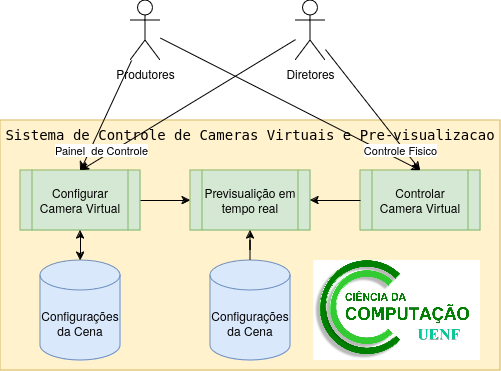
\includegraphics[width=0.8\textwidth]{Cameras}
    \caption{Diagrama de Interação Diretor com Sistema de cameras}
    \label{fig:diagram1}
\end{figure}

\subsection{Caso de Uso 2: Edição e Renderização de Vídeos}
\begin{description}[style=nextline]
    \item[Descrição:] Os editores utilizam este caso de uso para editar, ajustar efeitos visuais e renderizar vídeos usando os computadores de alta performance conectados ao servidor central. Os arquivos grandes são transmitidos diretamente do servidor para facilitar o trabalho.
    
    \item[Atores:] Editores de vídeo.
    
    \item[Pré-condição:] Os arquivos de vídeo e efeitos visuais estão disponíveis no servidor central.
    
    \item[Sequência de Ações:]
    \begin{enumerate}
        \item Acessar o sistema de edição.
        \item Carregar os arquivos de vídeo e efeitos necessários.
        \item Realizar a edição, incluindo cortes, ajustes e aplicação de efeitos.
        \item Iniciar a renderização do vídeo.
        \item Salvar o vídeo finalizado no servidor central.
    \end{enumerate}
    
    \item[Pós-condição:] O vídeo final está pronto para ser enviado ao cliente ou arquivado.
\end{description}

\begin{figure}[ht]
    \centering
    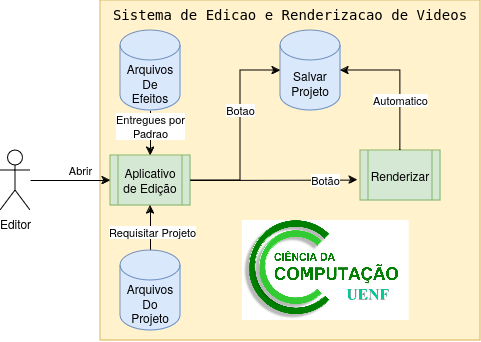
\includegraphics[width=0.8\textwidth]{Editores}
    \caption{Diagrama de Interação Editor Sistema}
    \label{fig:diagram1}
\end{figure}

\subsection{Caso de Uso 3: Gerenciamento de Projetos}
\begin{description}[style=nextline]
    \item[Descrição:] Este caso de uso permite o controle e acompanhamento de projetos no sistema. O cliente pode acessar um site interno para ver o progresso do projeto, dar feedback, e visualizar atualizações diretamente.
    
    \item[Atores:] Gerente de Projetos, Cliente.
    
    \item[Pré-condição:] O projeto está registrado no sistema com acesso disponível para o cliente.
    
    \item[Sequência de Ações:]
    \begin{enumerate}
        \item O gerente de projetos atualiza o status do projeto no sistema.
        \item O cliente acessa o site interno para verificar o andamento do projeto.
        \item O cliente visualiza o progresso, dá feedback e faz marcações se necessário.
        \item O gerente de projetos visualiza o feedback e atualiza o projeto conforme solicitado.
    \end{enumerate}
    
    \item[Pós-condição:] O projeto é atualizado de acordo com o feedback do cliente e segue para as próximas etapas.
\end{description}

\begin{figure}[ht]
    \centering
    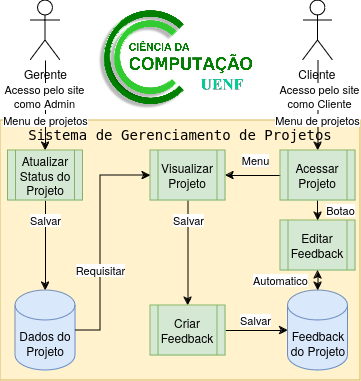
\includegraphics[width=0.8\textwidth]{Clientes}
    \caption{Diagrama de Interação Cliente/Gerente Sistema}
    \label{fig:diagram1}
\end{figure}

\pagebreak
\newpage

\section{Modelagem do Sistema}

Esta seção descreve a modelagem do sistema, incluindo a estruturação de dados e os processos principais. A modelagem de dados representa a estrutura e o armazenamento de informações, enquanto a modelagem de processos detalha o fluxo de dados e operações nos subsistemas principais.

\subsection{Modelagem de Processos: Subsistema de Edicao e Renderizacao de Videos}
O subsistema de edição e renderização lida com a aplicação de efeitos e o processamento dos vídeos. Ele permite que editores carreguem e modifiquem arquivos de vídeo.

\begin{itemize}
    \item \textbf{Dados de Entrada}: Arquivos de vídeo brutos, configurações de efeitos visuais.
    \item \textbf{Processos}:
        \begin{itemize}
            \item \textbf{Aplicar Efeitos}: O editor aplica efeitos visuais, com as configurações sendo carregadas e aplicadas ao vídeo.
            \item \textbf{Renderizacao de Video}: Após os efeitos, o vídeo é renderizado e salvo no servidor.
        \end{itemize}
    \item \textbf{Dados de Saída}: Vídeo finalizado, pronto para visualização ou download.
\end{itemize}

\subsection{Modelagem de Processos: Subsistema de Gerenciamento de Feedback e Progresso}
O subsistema de gerenciamento de feedback e progresso armazena as atualizações de projetos e feedbacks dos clientes, permitindo o acompanhamento contínuo dos editores.

\begin{itemize}
    \item \textbf{Dados de Entrada}: Atualizações do gerente de projetos, feedback do cliente.
    \item \textbf{Processos}:
        \begin{itemize}
            \item \textbf{Atualizacao de Progresso do Projeto}: O gerente atualiza o status do projeto, que é salvo no banco de dados.
            \item \textbf{Registro de Feedback do Cliente}: Clientes fornecem feedback sobre os vídeos, o qual é armazenado.
        \end{itemize}
    \item \textbf{Dados de Saída}: Relatórios de progresso e feedback do cliente.
\end{itemize}

\subsection{Modelagem de Processos: Subsistema de Gerenciamento de Recursos de Projeto}
Este subsistema gerencia os arquivos e recursos do projeto, organizando e armazenando arquivos multimídia e dados relacionados ao projeto.

\begin{itemize}
    \item \textbf{Dados de Entrada}: Arquivos de mídia brutos, metadados do projeto.
    \item \textbf{Processos}:
        \begin{itemize}
            \item \textbf{Armazenamento de Arquivos}: Os arquivos carregados são armazenados no sistema de arquivos e referenciados na base de dados.
            \item \textbf{Catalogacao de Recursos}: Os metadados dos recursos são organizados e catalogados para facilitar o acesso durante o processo de edição.
        \end{itemize}
    \item \textbf{Dados de Saída}: Recursos organizados e prontos para uso nas etapas de edição e renderização.
\end{itemize}

\subsection{Modelagem de Dados}

\begin{itemize}
  \item DER-01

  \item DER-02

  \item DER-03

  \item DER-04

\end{itemize}

